\scanpage{22}
\diagram{\begin{tikzcd}[ampersand replacement=\&,column sep=1em,row sep=.7em]
\pi_1G=\mathrm{Ker}\,( \& \pi_1(H)\arrow[r,""{name=k,coordinate}]\arrow[dd,""{name=v,coordinate}] \& \pi_0N\arrow[d,equal] \\
\phantom{\partial} \& \& N\arrow[d,phantom,"{\cup}"]\\
\& \pi_0(\pi)=\pi\arrow[ur]\arrow[r,"\varphi"'] \& \mathfrak{z}(N)
\arrow[from=1-2,to=k,phantom,shift left=2ex,"{\text{(connu)}\downarrow}"]
\arrow[from=v,to=2-1,no head,thin,bend right=12,shorten >=1.5em]
\arrow[from=3-2,to=3-3,no head,thin,start anchor=south,end anchor=south,bend right=66,shorten >=.7em]
\end{tikzcd}}
\margin{[\(\partial\) associé à suite exacte d'homotopie pour ext. \(1\to\pi\to\widetilde H\to H\to1\)]}
\margin{Car \(\pi\) discret}

\deleted{\unsure{et}} et on a
\diagram{\begin{tikzcd}[ampersand replacement=\&,column sep=1.1em,row sep=1em]
\pi_1H\arrow[r,"{\text{connu}\,\downarrow}"]\arrow[d,"\partial"'] \& N\arrow[r] \& \pi_0G\arrow[r] \& \pi_0H\arrow[r]\&1\\
\pi\arrow[r,"\varphi"] \& \mathfrak{z}(N)\arrow[u,hook] \& \&\&
\end{tikzcd}}
i.e. \(\pi_0G\deleted{\unsure{{}_0}}\) est une extension de \(\pi_0H\) par \(\mathrm{Coker}\,(\pi_1H\to N]\). Or on a une extension \(G_0\) de \(\unsure{\mathfrak{S}|\mathcal{G}|\mathfrak{G}}\) par \(N\) d'où, grâce à \(H\to\mathfrak{S}\) \inserted{(défini car \(\pi\subset\widetilde H_0\))} (i.e. \(\pi_0H\to\mathfrak{S}\) (\(=\pi_0\mathfrak{S}\)) car \(\mathfrak{S}\) discret) une extension \(G_1\) de \(\pi_0H\) par \(\deleted{\mathfrak{S}}N\) ;

% slanted
\margin{\rotatebox{30}{faux}\quad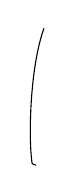
\begin{tikzpicture}[baseline]\draw[thin] (0,.6) .. controls (-.18,.1) and (-.20,-.8) .. (-.15,-1.12) -- (-.10,-1.14);\end{tikzpicture}}
On vérifie alors qu'on a
\diagram{\begin{tikzcd}[ampersand replacement=\&,column sep=.65em,row sep=.6em]
\pi_0G\simeq\mathrm{Coker}\,( \& \pi_1H\arrow[r]\arrow[dd,"\partial"] \& G_1\arrow[d,phantom,"\cup"]\& )\\
\& \& N\arrow[d,phantom,"\cup"]\&\\
\& \pi\arrow[r,"\varphi"] \&\mathfrak{z}(N)\&
\end{tikzcd}}
% archive sheet number: 21

